As the goal is to attempt to verify the Jeffrey equations in eq \ref{eq:jeffrey} we need an experimental setup with particles and flow system that satisfy the conditions that the Jeffrey equations apply under. This means our particles have to be bouyant,triaxially symmetric and small enough that inertial effects are not a problem. The flow has to be a linear creeping flow, in other words have a Reynolds number satisfying $Re << 1$ but have a high unidirectional shear that allows one to detect the orbits in a finite distance.

% Change the citation to the paper from anton thesis

The particles used in previous measurements were made from apoxy \cite{exjobb:anton} which made them buoyant and small enough to ignore inertial effects, but they were not symmetrical enough to produce reliable periodic Jeffrey orbits. Thus two sets of glass particles from Nippon Glass, Japan\cite{particles}, have been used. They are cylindrical with a consistent width of \unit[3]{$\mu$m} and \unit[5]{$\mu$m} and varying length. 

% Inclue pictures of particles and shit here

However they are made glass with a density of approximately \unit[2.57]{g/cm$^3$} at \unit[20]{C$^\circ$} which is significantly higher than that of water with a density of \unit[1]{g/cm$^3$} at \unit[20]{C$^\circ$} and glycerol with a density of \unit[1.5]{g/cm$^3$}. Thus to correct for the density and limit sinking or floating the water soluble Sodium metatungstate which at \unit[20]{C$^\circ$} has maximum density of \unit[2.94]{g/cm$^3$}. To increase the viscosity of the liquid around 8\% glycerol is added, resulting in a measured dynamic viscosity of \unit[$24\cdot 10^{-3}$]{Pa s}

% PIcture of the channel meassurements here 

This liquid with suspended particles is flowed through a channel of Polydimethylsiloxane (PDMS) \unit[4]{cm} long, \unit[2.5]{mm} wide and either \unit[200]{$\mu$m} and \unit[500]{$\mu$m}. The flow profile of such a channel was calculated by Anton Johansson in his thesis\cite{AntonThesis} and can be seen in figure \ref{}. The flow rate varies between $2$ and \unitfrac[20]{$\mu$l}{m} or in SI units \unitfrac[$3.33\cdot 10^-10$]{m$^3$}{s} which with a cross section of at least \unit[$5\cdot 10^-7$]{m^2}means a maximum flow speed of \unitfrac[6.66]{mm}{s}.

% Picture of channel flow profile


To confirm that the flow is a creeping flow we can calculate the maximum Reynolds number using eq \ref{eq:reynolds} and our maximum flow speed 

\begin{equation}
Re = \frac{U L \rho}{\mu} 
\leq \frac{6.66\cdot 10^{-3} \cdot 2.5 \cdot 10^{-3} 2.5 }{24 \cdot 10^{-3}} 
\approx	 	1.6  \cdot 10^{-3} \ll 1
\end{equation}

This should satisfy the conditions of the Jeffrey equations. To track the particles the channel is put in a moveable stage on a confocal microscope. The entire setup can be seen in figure \ref{fig:experimentalsetup}

\begin{figure}
\begin{center}
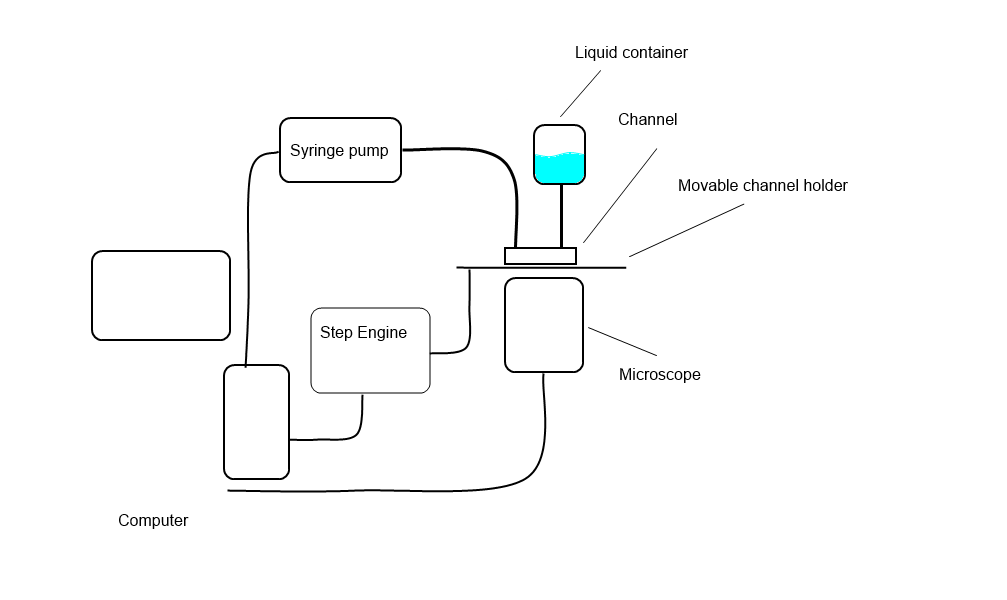
\includegraphics[width=0.7\textwidth]{figures/setupsketch.png}
\end{center}
\caption{}
\label{}
\end{figure}








In order to study the dynamics of particles, a channel made from PDMS and bonded onto a glass slide. A fluid containing the triaxial glass particles that can be seen in fig re REF HERE is pumped at a constant rate through the channel using a INSERT THE PUMP NAME HERE. To observe the particles, the channel is placed upon a confocal microscope connected to a INSERT CAMERA MODEL HERE. The channel is then moved using a INSERT STEP ENINE NAME HERE controlled from a computer. A mroe detailed description of the setup can be seen in figure REF to SETUP IMAGE THAT I MAKE

\section{The particles}
	Previously the particles used in the experiment were polymeric made by swirling an apoxy solution in a vortex. This produces rod like particles of different lengths, but very often included noticeable defects such as being bent, small lumps etc. 
	
	To improve results glass particles from Nippon Glass company in Japan were brought in. As they are mainly manufactured to serve as spacing rods in LCD screens they have a very well determined width but then broken at varying lengths. These breaking points are the only real visible point of imperfection of the rods.
	The specification of length and width can be seen in figure \ref{fig:rod_lengths}
	
	While the glass rods are far more regular in terms of size and shape, they do have on major problem. The density of the glass is \unitfrac[2.57]{g}{cm$^3$}, significantly higher than water which has a density of around $\unit[1]{g/cm}$ at 20 degrees C and glycerol which has a density of DENSITY OF GLYCEROL. And so the particles sink very quickly in any mix of water and glycerol.
	
	The solution is to use Sodium Metatungstate, a water soluble mineral which gives the resulting mix a maximum density of around $\unit[3]{g/cm}$ which is more than sufficient to keep the particles suspended. However the viscocity of only water and Sodium Metatungstate is only around  SOMETHING OR OTHER

	
	
	
\subsection{Density matching}

I guess we use sodium meta tungstate. But does this really need a whole section? Seems like overdoing it... but what %else have I done v_v
THE EQUATION FOR MODIFYING VISCOCITY

\begin{equation}
\rho_{a} = 	\frac {m_{a}}{V_{a}} =
				\frac{V_{b}\rho_{b} + V_{mix}\rho_{mix}}{V_b + V_{mix}} 
\end{equation}
So if we want to find $V_{mix}$ we get
\begin{equation}
V_{mix} = \frac{ V_{b}(\rho_{b} - \rho_{a})}{\rho_{a} - \rho_{mix}} 
\end{equation}

